\fancyhead[L]{\textbf{\large 10}\quad\sffamily\textbf{\color{darkgray}CHƯƠNG 1}\quad\sffamily\color{darkgray}Hàm số và Mô hình}
\fancyhead[R]{}

\noindent
\begin{minipage}[t]{0.26\textwidth}
    \vspace{1.48cm}
    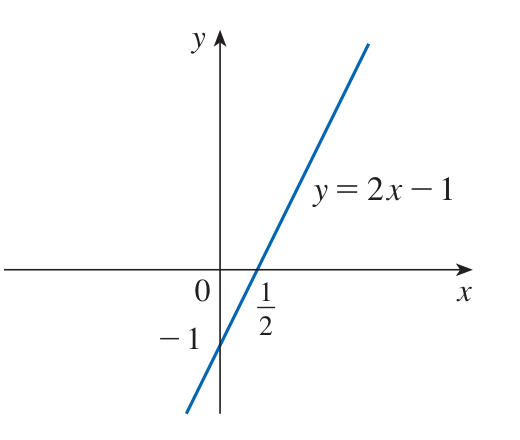
\includegraphics[width=\linewidth]{images/figure_7_clean.png}\\[2pt]
    {\small\textbf{\textsf{HÌNH 7}}}

    \vspace{1.48cm}
    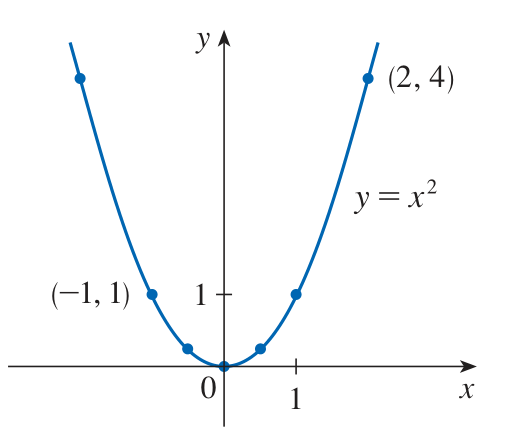
\includegraphics[width=\linewidth]{images/figure_8_clean.png}\\[2pt]
    {\small\textbf{\textsf{HÌNH 8}}}

    \vspace{1.8cm}
    {\footnotesize Biểu thức
    \[
    \frac{f(a+h) - f(a)}{h}
    \]
    trong Ví dụ 3 được gọi là \textbf{thương sai phân} (\textit{difference quotient}) và xuất hiện rất thường xuyên trong giải tích. Như chúng ta sẽ thấy trong Chương 2, nó biểu thị tốc độ biến thiên trung bình của hàm số $f(x)$ giữa $x = a$ và $x = a + h$.}
\end{minipage}%
\hfill
\begin{minipage}[t]{0.71\textwidth}
    Trong giải tích, phương pháp phổ biến nhất để xác định một hàm số là thông qua một phương trình đại số. Ví dụ, phương trình $y = 2x - 1$ xác định $y$ là một hàm số theo $x$. Ta có thể biểu diễn hàm này dưới dạng ký hiệu hàm số là $f(x) = 2x - 1$.

    \vspace{0.2cm}
    \noindent{\large\textbf{\textsf{\color{stewartcyan}VÍ DỤ 2}}}\quad Vẽ đồ thị, đồng thời tìm tập xác định và tập giá trị của mỗi hàm số sau:
    \vspace{-0.1cm}
    \begin{center}
        \textbf{(a)}\quad $f(x) = 2x - 1$ \qquad\qquad \textbf{(b)}\quad $g(x) = x^2$
    \end{center}

    \noindent{\textbf{\textsf{\color{stewartcyan}LỜI GIẢI}}}

    \textbf{(a)} Phương trình của đồ thị là $y = 2x - 1$, và ta dễ dàng nhận ra đây là phương trình của một đường thẳng có hệ số góc bằng $2$ và tung độ gốc bằng $-1$. (Hãy nhớ lại dạng phương trình đường thẳng theo hệ số góc và tung độ gốc: $y = mx + b$. Xem Phụ lục B.) Điều này cho phép chúng ta phác thảo một phần đồ thị của hàm số $f$ như trong Hình 7. Biểu thức $2x - 1$ xác định với mọi số thực, do đó tập xác định của $f$ là tập hợp tất cả các số thực, ký hiệu là $\mathbb{R}$. Đồ thị cũng cho thấy tập giá trị của hàm số là $\mathbb{R}$.

    \textbf{(b)} Vì $g(2) = 2^2 = 4$ và $g(-1) = (-1)^2 = 1$, ta có thể chấm các điểm $(2, 4)$ và $(-1, 1)$ cùng với một vài điểm khác trên hệ trục tọa độ, sau đó nối các điểm lại để tạo thành đồ thị (Hình 8). Phương trình của đồ thị là $y = x^2$, biểu diễn một đường parabol (xem Phụ lục C). Tập xác định của $g$ là $\mathbb{R}$. Tập giá trị của $g$ bao gồm tất cả các giá trị của $g(x)$, tức là tất cả các số có dạng $x^2$. Nhưng $x^2 \ge 0$ với mọi số $x$, và mọi số dương $y$ đều là bình phương của một số nào đó. Do đó, tập giá trị của hàm số $g$ là $\{y \mid y \ge 0\} = [0, \infty)$. Điều này cũng được thể hiện trực quan trên Hình 8. \hfill {\color{stewartcyan}$\blacksquare$}

    \vspace{0.29cm}
    \noindent{\large\textbf{\textsf{\color{stewartcyan}VÍ DỤ 3}}}\quad Nếu $f(x) = 2x^2 - 5x + 1$ và $h \ne 0$, hãy tính giá trị của biểu thức $\dfrac{f(a + h) - f(a)}{h}$.

    \vspace{0.12cm}
    \noindent{\textbf{\textsf{\color{stewartcyan}LỜI GIẢI}}}\quad Trước tiên, ta tính $f(a + h)$ bằng cách thay $x$ bởi $a + h$ vào biểu thức của $f(x)$:
    \begin{align*}
    f(a + h) &= 2(a + h)^2 - 5(a + h) + 1 \\
    &= 2(a^2 + 2ah + h^2) - 5(a + h) + 1 \\
    &= 2a^2 + 4ah + 2h^2 - 5a - 5h + 1
    \end{align*}
    Sau đó, ta thế vào biểu thức đã cho và rút gọn:
    \begin{align*}
    \frac{f(a + h) - f(a)}{h} &= \frac{(2a^2 + 4ah + 2h^2 - 5a - 5h + 1) - (2a^2 - 5a + 1)}{h} \\
    &= \frac{2a^2 + 4ah + 2h^2 - 5a - 5h + 1 - 2a^2 + 5a - 1}{h} \\
    &= \frac{4ah + 2h^2 - 5h}{h} = 4a + 2h - 5 \qquad {\color{stewartcyan}\blacksquare}
    \end{align*}

    \vspace{0.16cm}
    \noindent{\large\textbf{\textsf{\color{stewartcyan}■ Các biểu diễn của hàm số}}}
    \vspace{0.12cm}

    Chúng ta xem xét bốn phương pháp khác nhau để biểu diễn một hàm số:
    \begin{itemize}[itemsep=0.08cm, topsep=0.1cm]
        \item[{\color{stewartred}\textbullet}] \textbf{bằng lời} \qquad\qquad\quad\ (mô tả bằng câu chữ)
        \item[{\color{stewartred}\textbullet}] \textbf{bằng số liệu} \qquad\qquad\ (bằng một bảng giá trị)
        \item[{\color{stewartred}\textbullet}] \textbf{bằng hình ảnh trực quan} \ (bằng đồ thị)
        \item[{\color{stewartred}\textbullet}] \textbf{bằng đại số} \qquad\qquad (bằng một công thức giải tích tường minh)
    \end{itemize}

    Nếu một hàm số có thể được biểu diễn bằng cả bốn phương pháp trên, việc chuyển đổi linh hoạt qua lại giữa các cách biểu diễn sẽ mang lại cái nhìn sâu sắc hơn về bản chất của hàm số đó. Tuy nhiên, một số hàm số nhất định lại được mô tả tự nhiên hơn bằng phương pháp này thay vì phương pháp khác. Với tinh thần đó, chúng ta hãy cùng xem xét lại bốn tình huống đã nêu ở phần mở đầu của mục này.
\end{minipage}